\section{Multivariable Integral Calculus}

\subsection{Function Not Satisfying Fubini's Theorem}

\subsubsection*{Set Up}

Here we consider Fubini's theorem in two-dimensions.

Fubini's theorem tells us two things:
\begin{itemize}
\item When we know we can compute a two-dimensional integral as a repeated application of one-dimensional integration over the variables \(x\) and \(y\).

\item When we know the order of the repeated one-dimensional integration over \(x\) and \(y\) doesn't depend on the order of integrating over \(x\) and \(y\). 

\end{itemize}

We will consider the problem of finding a simple function that doesn't satisfy Fubini's theorem. In particular, the result of applying the repeated 
one-dimensional integration will depend on the order of \(x\) and \(y\). We will aim to find a simple elementary function, and we will keep the domain of integration
simple, i.e. the square \(S = \{0 \leq x \leq 1 \text{ and } 0 \leq y \leq 1\}\).

As a hint as to how this process will work, let us recall the fact that for a convergent series \(\sum_i a_i\), the limit of the partial sums is independent of the order of
the sum when the series is absolutely convergent, i.e. \(\sum_i |a_i| < \infty\). For our problem of finding an appropriate function \(u(x,y)\), we are then lead to consider
finding a function \(u(x,y)\) that satisfies the following:
\begin{itemize}
\item The function \(u(x,y)\) takes positive and negative values. 
\item The integral of the aboslute value of \(u\) is not convergent, i.e. \(\iint_s |u| \dA = \infty\).
\item The integrals of the positive and negative parts of the function must cancel out in some way such that the repeated integration gives nice finite values despite
the fact that \(\iint_s |u| \dA = \infty\).
\end{itemize}


\subsubsection*{The Problem}

Find a nice elementary function \(u(x, y)\) defined on the square \(s = \{0 \leq x \leq 1 \text{ and } 0 \leq y \leq 1\}\) such that \(u(x,y)\) doesn't satisfy Fubini's theorem in the following sense:
\begin{itemize}
\item Both of the repeated integrals
\begin{equation}
\int\limits_0^1 \int\limits_0^1 u(x,y) \dx \dy,
\end{equation}
and
\begin{equation}
\int\limits_0^1 \int\limits_0^1 u(x,y) \dy \dx,
\end{equation}
exist and are finite.
\item However, the repeated integrals mentioned above are NOT equal.
\end{itemize}

\subsubsection*{Solution}

To keep things simple, we find a function \(u(x,y)\) that blows up to both \(\pm \infty\) at the corner \((0,0)\). First let us observe that the function 
\begin{equation}
f(x,y) = \frac{-1}{(x+y)^2}
\end{equation}
has \(\iint_S |f| \dA = \infty\); you can quickly see that convergence of this integral is suspect because \(|f|\) of order \(r^{-2}\) as the radius \(r \to 0\). This is the edge case of convergence
for two-dimensions (recall that the area element for polar coordinates in two-dimensions includes an extra \(r\), i.e. \(\dA = r d\theta dr\)). 

However, \(f(x,y)\) is always negative inside the square \(S\); so we won't get the cancellation of positive and negative parts that we desire. To fix this we set up \(u(x,y)\) to be a difference
of \(f(x,y)\) and a similar function. First, let \(A, B\) be constants that we will determine later. Then we use
\begin{equation}
u(x,y) = \frac{1}{(Ax + By)^2} - \frac{1}{(x+y)^2} .
\end{equation}

We need that \(u\) takes positive and negative values in \(S\). To make sure \(u\) is always defined in \(S\) we will restrict to considering \(A, B > 0\).

Next, consider the values of \(u\) along the line \(\{x + y = 1\}\). This line joins two corners of \(S\), i.e. \((0,1)\) and \((1,0)\). We will design \(A\) and \(B\) to make
sure \(u\) has opposite signs at these two corners. To do so, we need to compare the sizes of \(Ax + By\) and \(x + y\) at these two corners.

To get opposite signs, we need that \(Ax + By\) is above \(1\) at one of these two corners and below \(1\) at the other corner. At \((0,1)\), \(Ax + By = B\) and at \((1,0)\), \(Ax + By = A\).
So we can choose \(A\) is above \(1\) and \(B\) is below \(1\). A convenient choice is \(A = 2\) and \(B = 1/2\) (if you dive deeper into the construction, you will find that the reciprocal nature of \(A\) and \(B\) is also necessary, but we won't go into detail on this). 

So we have that
\begin{equation}
u(x,y) = \frac{1}{(2x + y/2)^2} - \frac{1}{(x+y)^2}.
\end{equation}
Let us verify that this function \(u(x,y)\) satisfies the conditions on the repeated integrals that we are looking for.

First, note that for any \(y > 0\), we have
\begin{align}
\int\limits_0^1 \frac{1}{(2x + y/2)^2} - \frac{1}{(x+y)^2} \dx & = \left.\frac{1}{x+y} - \frac{1}{2(2x + y/2)}\right|^1_{x = 0}, \\ 
    & = \frac{1}{1 + y} - \frac{1}{y} - \frac{1}{4+y} + \frac{1}{y}, \\
    & = \frac{1}{1+y} - \frac{1}{4+y}.
\end{align}
So we get that
\begin{align}
\int\limits_0^1 \left(\int\limits_0^1 \frac{1}{(2x + y/2)^2} - \frac{1}{(x+y)^2} \dx\right) \dy & = \int\limits_0^1 \frac{1}{1+y} - \frac{1}{4 + y} \dy, \\
    & = \left. \log(1 +y) - \log(4 + y)\right|_{y = 0}^1, \\
    & = \log(2) - \log(1) - \log(5) + \log(4), \\
    & = 3\log(2) - \log(5). 
\end{align}

Now, let us consider the other iterated integral. First, for any \(x > 0\), we have that
\begin{align}
\int\limits_0^1 \frac{1}{(2x + y/2)^2} - \frac{1}{(x+y)^2} \dy & = \left.\frac{1}{x+y} - \frac{2}{2x + y/2}\right|_{y = 0}^1, \\
    & = \frac{1}{x+1} - \frac{1}{x} -\frac{2}{2x+1/2} + \frac{2}{2x}, \\ 
    & = \frac{1}{x+1} - \frac{2}{2x+1/2}.
\end{align}
So we have that
\begin{align}
\int\limits_0^1 \left(\int\limits_0^1 \frac{1}{(2x + y/2)^2} - \frac{1}{(x+y)^2} \dy\right) \dx & = \int\limits_0^1 \frac{1}{x+1} - \frac{2}{2x+1/2} \dx, \\
    & = \left. \log(x+1) - \log(2x + 1/2)\right|_{x = 0}^1, \\
    & = \log(2) - \log(1) - \log(5/2) + \log(1/2), \\
    & = \log(2) - \log(5). 
\end{align}
And so we see the repeated integrals are finite, but do NOT match.


%%%%%%%%%%%%%%%%%%%%%%%%%%%%%%%%%%%%%%%%%%%%%%%%%%%

\subsection{Interesting Property of Significands Under Multiplication}

\subsubsection*{The Setup}

Before we get started, let's explain the concept of the significand of a number(also sometimes referred to as the mantissa). Essentially, the significand of a
number is the collection of significant digits in scientific notation, which we will take to be normalized to be between 1 and 10. For example, the
significand of \(1059\) is \(1.059\), because \(1059 = 1.059 \times 10^3\) in scientific notation. So the significand is found by simply ignoring the exponent
in scientific notation. Note that the significand isn't defined for the number zero. 

Let us denote the signficand of a number \(x\) by \(s(x)\).

Now we consider the case that we have a distribution of random significands \(X\) such that their probability distribution is given by 
an inverse distribution. That is, the probability density is \(\frac{1}{x\log(10)}\), i.e. for any \(1 \leq x < 10\),
\begin{equation}
P\left(X \leq x\right) = \int \limits_1^x \frac{1}{s\log(10)} ds.
\end{equation}

We also assume we have another distribution of random significands \(Y\) such that their probability distribution is given by an 
arbitrary density \(f(y)\). That is, for any \(1 \leq y < 10\), we have 
\begin{equation}
P\left(Y \leq y\right) = \int \limits_0^y f(s) ds.
\end{equation}

We will consider the distribution of the significands for the product of \(X\) and \(Y\); that is \(P(s(XY) \leq z)\). Let \(h(z)\) be the density of the probability
distribution of \(s(XY)\). We will show that
\begin{equation}
h(z) = \frac{1}{z\log(10)}.
\end{equation}
That is, the significands of the products also have an inverse distribution, no matter what the density \(f(y)\) is. For a more detailed discussion, please see \cite{Hamming}.

Since we seek the distribution of a random variable that is real valued, it is helpful to consider the appropriate cumulative distribution. Since we denote the density of 
the signficands \(s(XY)\) by \(h(z)\), we will then let \(H(z)\) be the cumulative distribution, i.e. 
\begin{align}
H(z) & = P(1 \leq s(XY) \leq z) \\
    & = \int_1^z h(z) dz,
\end{align}
for any \(1 \leq z < 10\). Recall that the significand is always between 1 and 10.

Similary, we let \(F(y)\) be the cumulative distribution for \(f(y)\).

Next, let us describe which significands \(X\) and \(Y\) satisfy \(1 \leq s(XY) \leq z\). First, we have the case that the product satisfies \(XY < 10\). In this case, we have that
the significand \(s(XY) = XY\). However, in the case that \(XY \geq 10\), we have that \(s(XY) = XY / 10\); we need to divide by \(10\) to move the decimal point to the right. So we
see that
\begin{equation}
\{1 \leq s(XY) \leq z\} = \{1 \leq XY \leq z\} \cup \{10 \leq XY \leq 10z\}.
\end{equation}
Let \(U = \{1 \leq xy \leq z | 1\leq x,y < 10\}\) and \(V = \{10 \leq xy \leq 10z | 1\leq x, y < 10\}\).

Let's take a look at these regions.

\begin{figure}[h]
\centering
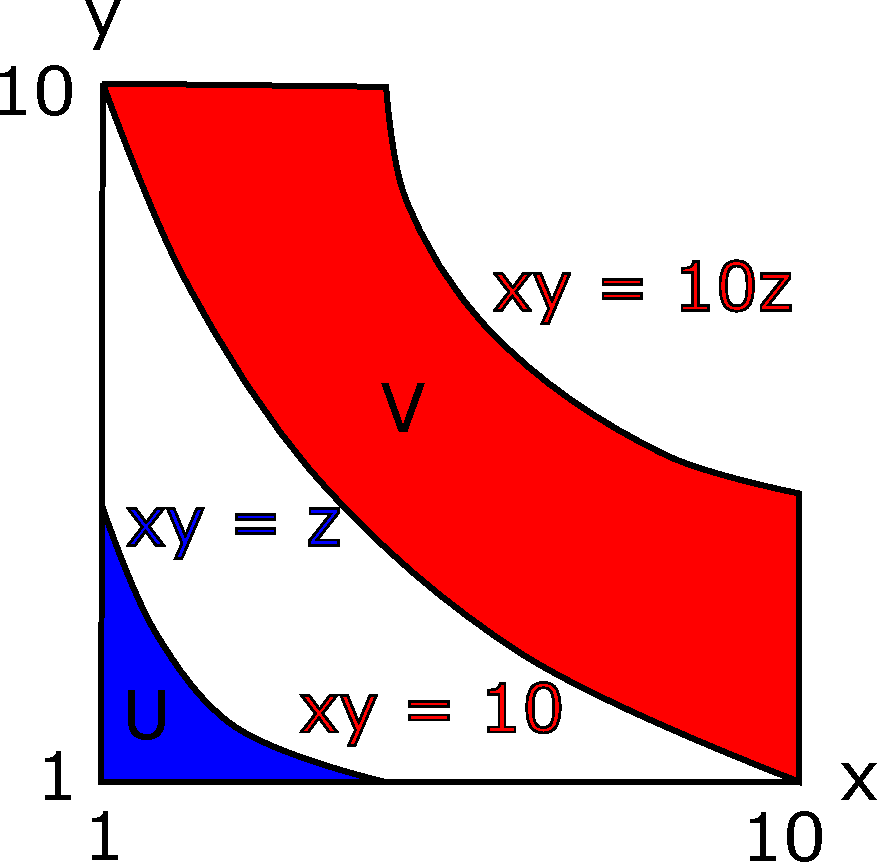
\includegraphics[width = 0.5\textwidth]{multiVarIntCalc/significandProduct.pdf}
\end{figure}

Let \(p(x,y)\) be the density for \((X, Y)\); we have that \(p(x,y) = \frac{f(y)}{x\log(10)}\). Then we have that our cumulative distribution is given by
\begin{align}
H(z) & = \iint\limits_{U\cup V} p(x,y) \dA_{xy}, \\ 
& = \frac{1}{\log(10)} \iint \limits_{U\cup V} \frac{f(y)}{x}  dA_{xy}.
\end{align}
We can use this expression for \(H(z)\) to compute the density \(h(z) = H'(z)\).

\subsubsection*{The Problem}

For \(1 \leq z < 10\), consider the regions \(U = \{1 \leq xy \leq z | 1 \leq x, y < 10 \}\) and \(V = \{10 \leq xy \leq 10z | 1 \leq x, y < 10\}\). Use that the
cumulative distribution \(H(z)\) satisfies 
\begin{equation}
H(z) = \frac{1}{\log(10)} \iint\limits_{U \cup V} \frac{f(y)}{x} \dA_{xy}, 
\end{equation}
to show that the density \(h(z) = H'(z)\) satisfies
\begin{equation}
h(z) = \frac{1}{z\log(10)},
\end{equation}
for \(1 \leq z \leq 10\).

\subsubsection*{The Solution}

Let us first compute \(H_U'(z)\) for \(H_U(z)\) defined by
\begin{equation}
H_U(z) \coloneqq \frac{1}{\log(10)} \iint\limits_U \frac{f(y)}{x}\dA_{xy}. 
\end{equation}
The region \(U\) is simple enough that we can compute this using iterated integrals. We have that
\begin{equation}
H_U(z) = \frac{1}{\log(10)}\int\limits_{1}^{z} \left( \int\limits_{1}^{z/x} \frac{f(y)}{x} dy\right) dx. 
\end{equation}
Now, we have that
\begin{equation}
\int\limits_{1}^{x/z} \frac{f(y)}{x} dy = \frac{1}{x} F\left(\frac{z}{x}\right).
\end{equation}
So,
\begin{equation}
H_U = \frac{1}{\log(10)}\int\limits_1^z \frac{1}{x} F\left(\frac{z}{x}\right) dx. 
\end{equation}
Therefore, using that \(F(1) = 0\) and a \(u\)-substitution, we have that
\begin{align}
H_U'(z) & = 0 + \frac{1}{\log(10)} \int\limits_1^z \frac{1}{x^2} f\left(\frac{z}{x}\right) dx, \\ 
    & = \frac{1}{z\log(10)} \int\limits_1^{z} f(u) du, \\
& = \frac{F(z)}{z\log(10)}.
\end{align}

Next, we compute \(H_V'(z)\) for \(H_V(z)\) defined by
\begin{equation}
H_V(z) \coloneqq \frac{1}{\log(10)} \iint\limits_V \frac{f(y)}{x}\dA_{xy}. 
\end{equation}
We can either compute this by breaking up the integral into regions where we can apply double iterated integrals or we can make a
change of coordinates. We will change our coordinates.

Define coordinates \(u = x\) and \(v = xy\); note that these are valid cooridinates for the square \(1 \leq x, y \leq 10\). In \(xy\)-coordinates,
the region \(V\) is specified by its four boundary pieces: \(\{x = 10\}\), \(\{y = 10\}\), \(\{xy = 10\}\), and \(\{xy = 10z\}\). In \(uv\)-coordinates,
these become \(\{u = 10\}\), \(\{v = 10u\}\), \(\{v = 10\}\), \(\{v = 10z\}\). Denote this tranformed region by \(\overline{V}\); below is a picture of \(\overline{V}\).

\begin{figure}[h]
\centering
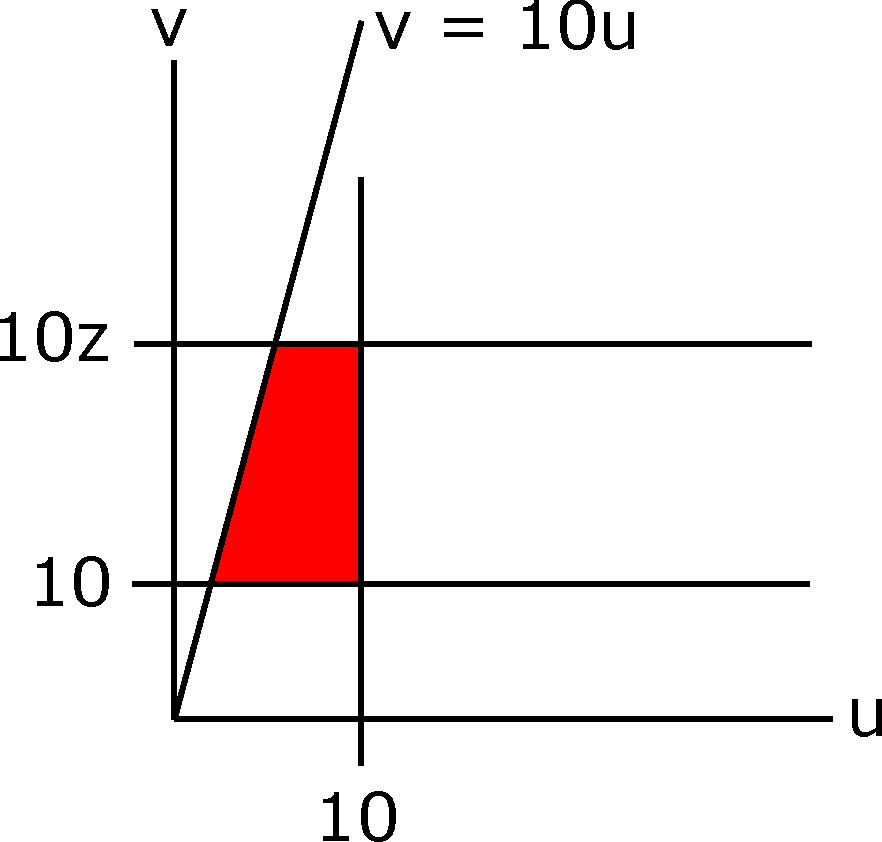
\includegraphics[width = 0.5\textwidth]{multiVarIntCalc/uvRegion.pdf}
\end{figure} 

We see that we can integrate over the region \(\overline{V}\) in the \(uv\)-plane with one application of iterated integrals. However,
first we need to compute the Jacobian factor for the transformation of coordinates. We have
\begin{equation}
\frac{\partial(u, v)}{\partial(x, y)} = x. 
\end{equation} 
So we get that
\begin{align}
\frac{\partial(x, y)}{\partial(u, v)} & = \frac{1}{x},\\
    & = \frac{1}{u}.
\end{align}
So we see that
\begin{align}
H_V(z) & = \frac{1}{\log(10)} \iint \limits_{\overline{V}} \frac{1}{u^2} f\left(\frac{v}{u}\right) dA_{uv}, \\
    & = \frac{1}{\log(10)} \int\limits_{10}^{10z} \left( \int\limits_{v/10}^{10} \frac{1}{u^2} f\left(\frac{v}{u}\right) du \right) dv.
\end{align}
For the inner integral we get
\begin{align}
\int\limits_{v/10}^{10} \frac{1}{u^2} f\left(\frac{v}{u}\right) du  & = \frac{1}{v} \int\limits_{v/10}^{10} f(w) dw, \\
    & = \frac{1}{v}\left(F(10) - F\left(\frac{v}{10}\right) \right), \\
    & =  \frac{1}{v}\left(1 - F\left(\frac{v}{10}\right) \right).
\end{align}
Here we have used that \(F(10) = 1\).

So then 
\begin{equation}
H_V(z) = \frac{1}{\log(10)} \int\limits_{10}^{10z} \frac{1}{v}\left(1 - F\left(\frac{v}{10}\right) \right) dv,
\end{equation}
and therefore
\begin{align}
H_V'(z) & = \frac{10}{10z\log(10)} \left(1 - F(z)\right), \\
    & = \frac{1}{z\log(10)} - \frac{1}{z\log(10)}F(z).
\end{align}
Since \(H(z) = H_U(z) + H_V(z)\), we have that \(h(z) = H_U'(z) + H_V'(z)\) and so we get 
\begin{equation}
h(z) = \frac{1}{z\log(10)}.
\end{equation}
